
\documentclass[8pt]{article}

\usepackage[utf8]{inputenc}

\usepackage{amsmath, bm}
\usepackage{graphicx}
\usepackage{amssymb}
\usepackage{float}
\usepackage{caption}
\usepackage{subcaption}
% set font size to 11pt

% set margin
\usepackage[margin=1in]{geometry}

\setlength{\parskip}{\baselineskip}%
\setlength{\parindent}{0pt}%
\setlength{\headsep}{5pt}

\begin{document}

% insert pdf cover page here


\title{Experimental Propeller Performance}
\author{lwp26}
\date{October 2024}
\maketitle

\section{Introduction}

A simple experimental setup was made to collect thrust and power data for different propeller designs.
The acoustic spectrum of the propellers was also crudely measured to identify sources of noise 


\section{Method}

The setup consisted of a motor on top of an automatically calibrating load cell, with a microphone held nearby.

Experiments with two motor controllers and three propeller designs were conducted.
The first controller used was an Odrive S1 which is a high performance motor controller, not designed for small quadcopter motors.
It has advanced features to measure input power and can provide velocity estimates obtained from the motors back EMF.
The second controller used was a LittleBee 30A ESC which also has a closed loop controller based on the back EMF, but lacks the ability to measure power or obtain the velocity estimate.

The motor was controlled in a staircase function where thrust and power are measured at the end of each step.
Points were also measured on the way down to measure hysteresis.
At the beginning of each run the thrust is automatically calibrated by automatically applying and releasing a known weight.

This weight was a 500ml water bottle which was weighed on some baking scales, accurate to 1g.
The setup was powered by a 3s 2400mAh LiPo battery, and so the voltage will change as the battery discharges.
For a complete uncertainty analysis it would be necessary to measure the battery voltage at the beginning and end of the experiment, but this was not done.

The microphone was connected to a picoscope to measure the spectrum of the noise generated by the propellers.
Spectrums were captured with the microphone approximately in the plane of the propellers at (unmeasured) high and low speeds.
A rough survey was done up to the axial direction to observe the directivity of the noise, the spectrums of which were not recorded.

\begin{figure}
    \centering
    
\includegraphics[width=0.99\textwidth]{figures/setup.jpg}
    \caption{Experimental setup showing propeller, motor, load cell and microphone}
    \label{fig:setup}
\end{figure}

\section{Results}

\begin{figure}[H]
    \centering
    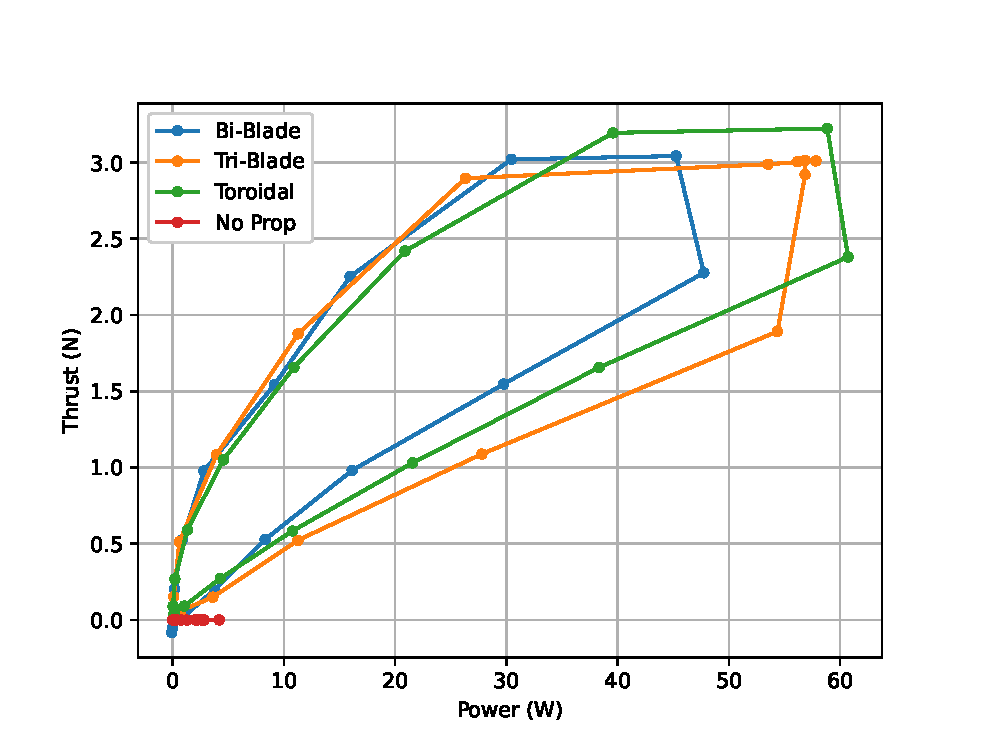
\includegraphics[width=0.99\textwidth]{figures/power_vs_thrust.eps}
    \caption{Measured Odrive power vs measured thrust}
    \label{fig:power_vs_thrust}
\end{figure}

\begin{figure}[H]
    \centering
    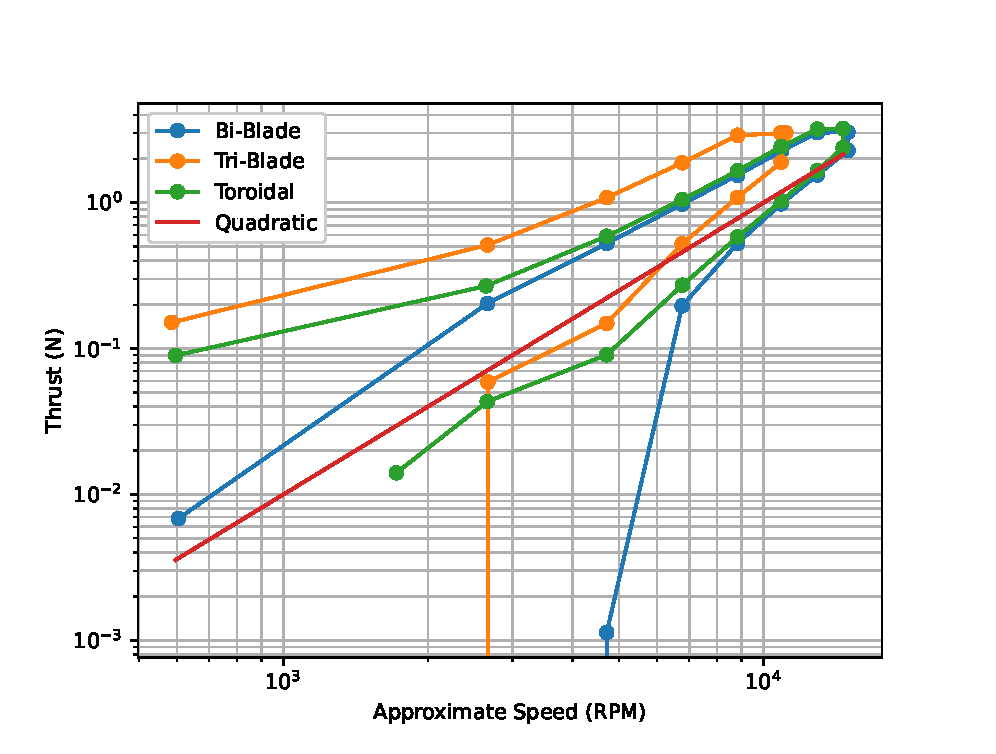
\includegraphics[width=0.99\textwidth]{figures/speed_vs_thrust.eps}
    \caption{Measured Odrive speed vs measured thrust}
    \label{fig:speed_vs_thrust}
\end{figure}

\begin{figure}[H]
    \centering
    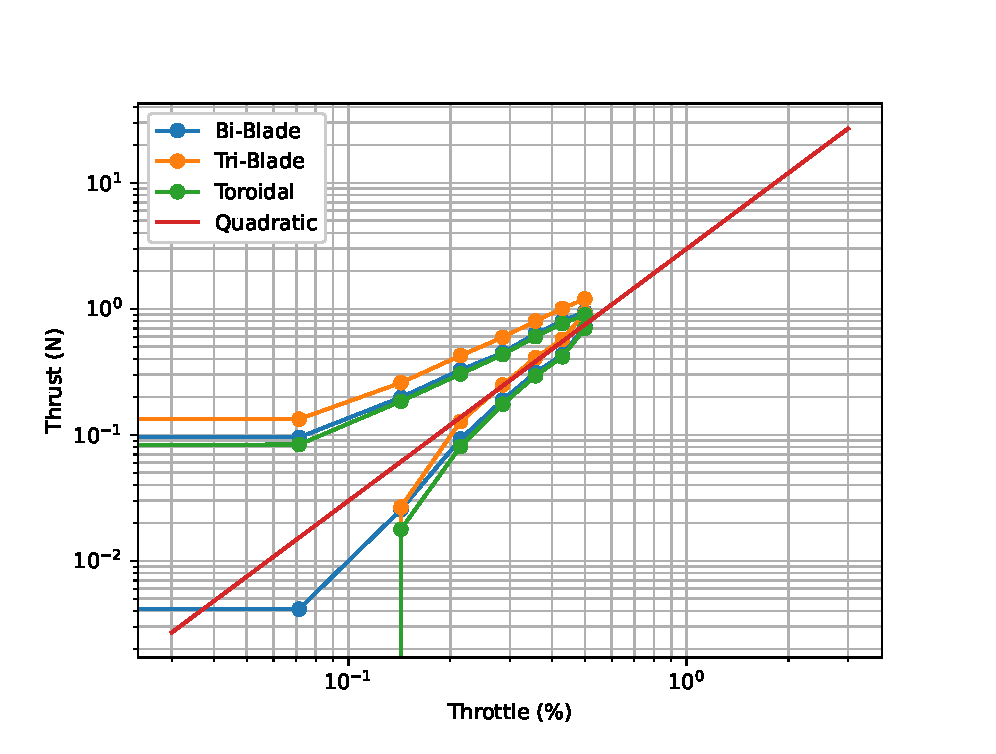
\includegraphics[width=0.99\textwidth]{figures/throttle_vs_thrust.eps}
    \caption{ESC input throttle vs measured thrust}
    \label{fig:throttle_vs_thrust}
\end{figure}

\begin{figure}[H]
    % subfigure
    \begin{subfigure}{0.99\textwidth}
        \centering
        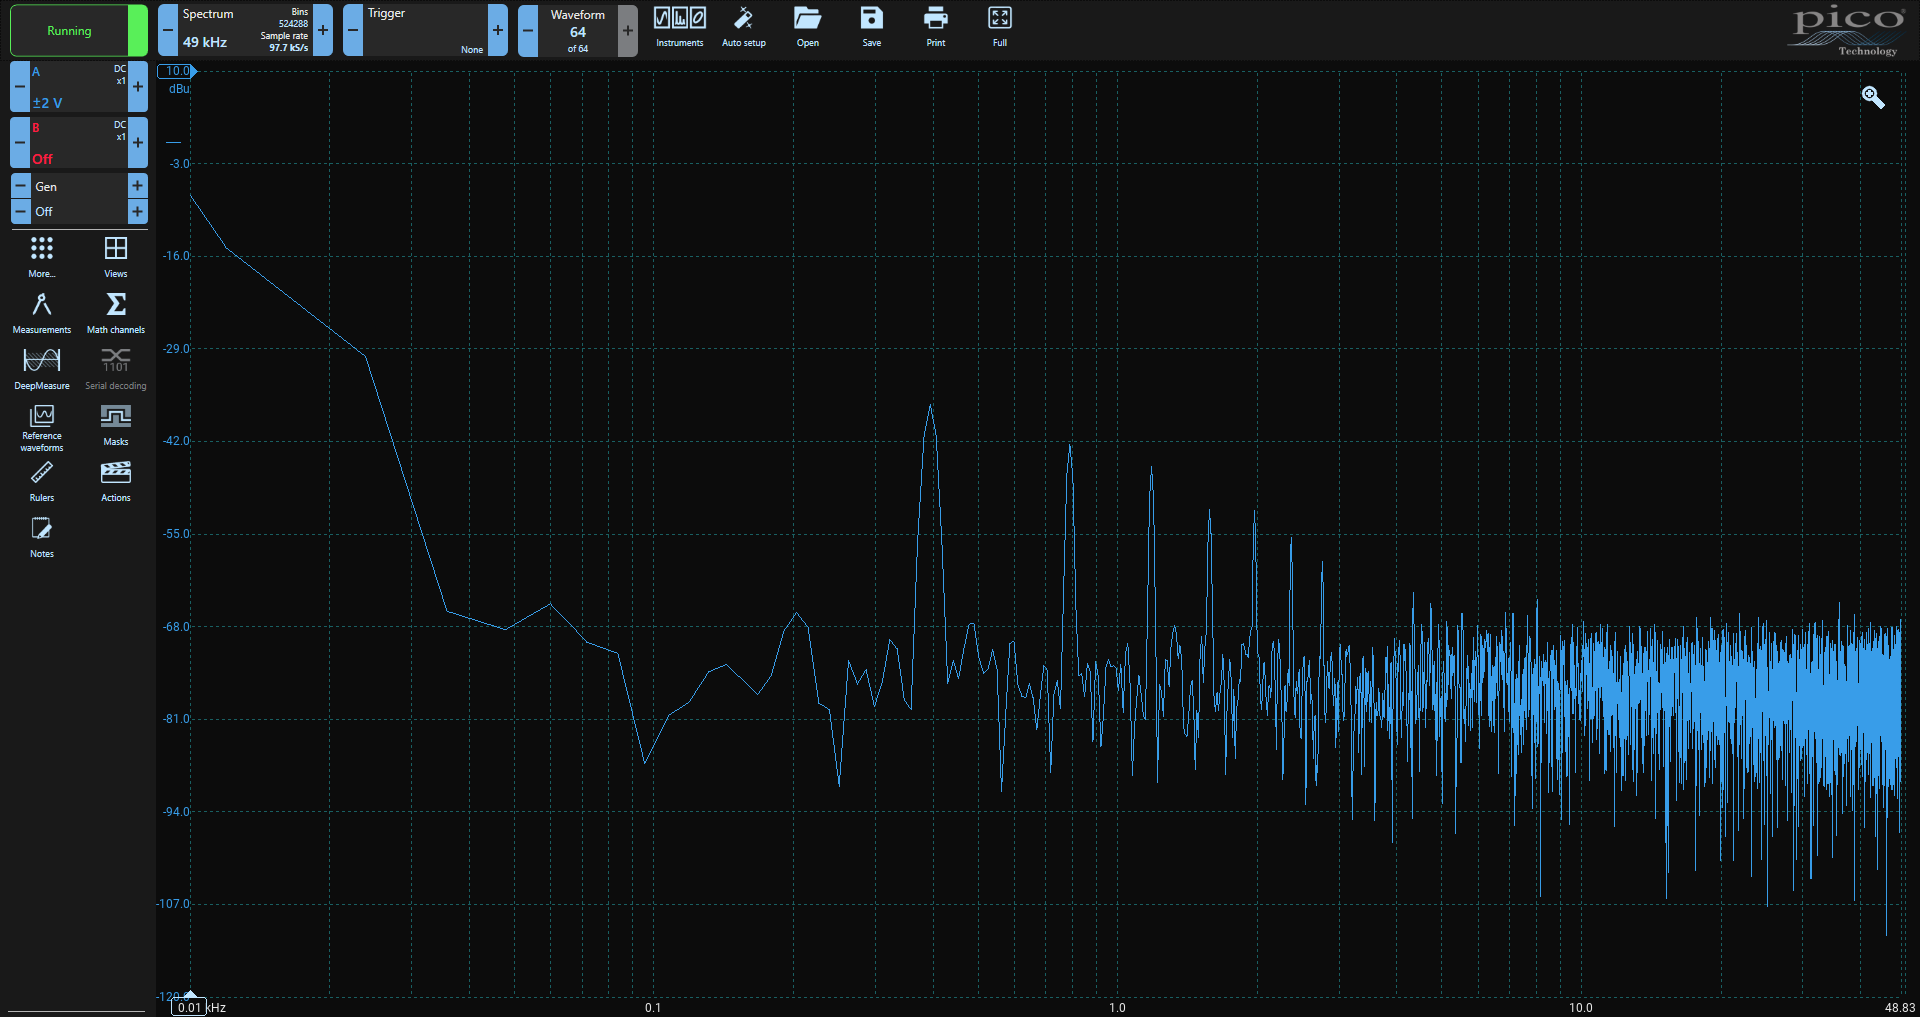
\includegraphics[width=0.99\textwidth]{figures/hispeed_biprop.png}
        \caption{Bi-Propeller}
        \label{fig:hispeed_biprop}
    \end{subfigure}
    % subfigure
    \begin{subfigure}{0.99\textwidth}
        \centering
        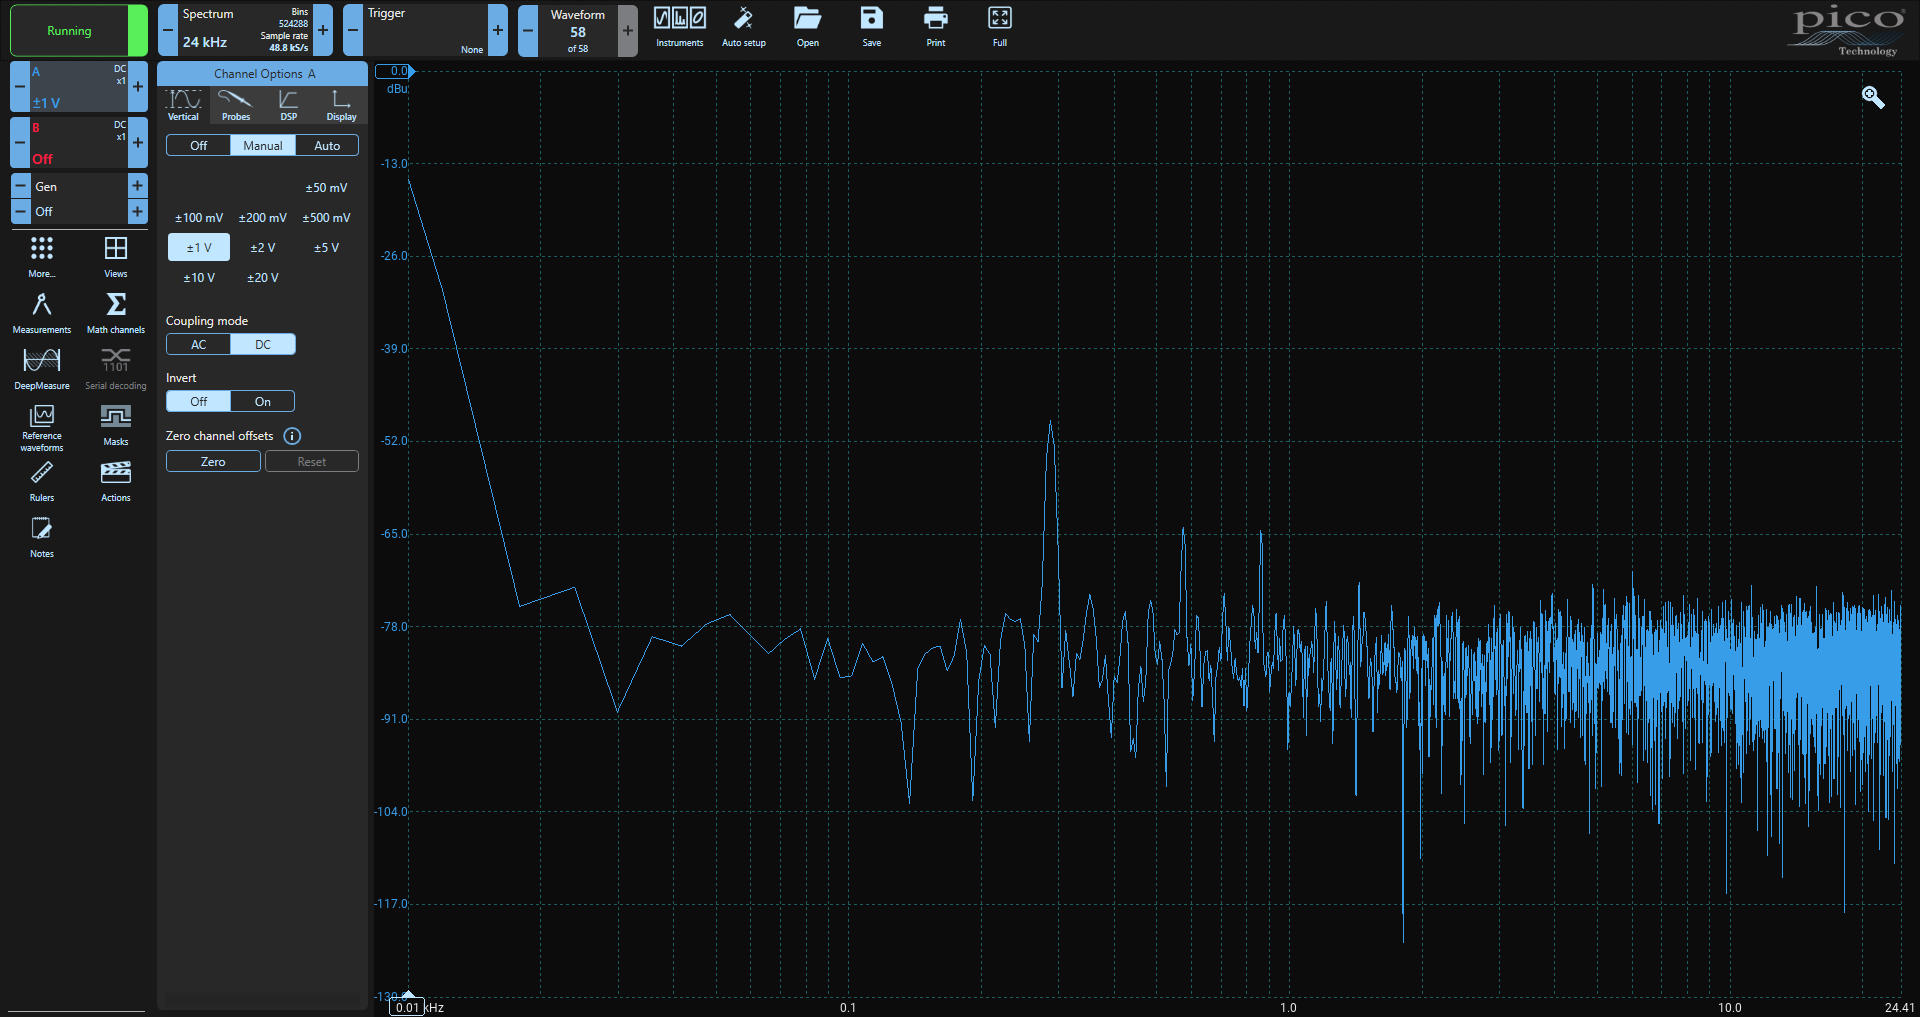
\includegraphics[width=0.99\textwidth]{figures/hispeed_toroid.png}
        \caption{Toroidal propeller}
        \label{fig:hispeed_toroid}
    \end{subfigure}
    \caption{Noise spectrum of propellers at high speed}
    \label{fig:noise_spectrum_hispeed}
\end{figure}

\begin{figure}[H]
    % subfigure
    \begin{subfigure}{0.99\textwidth}
        \centering
        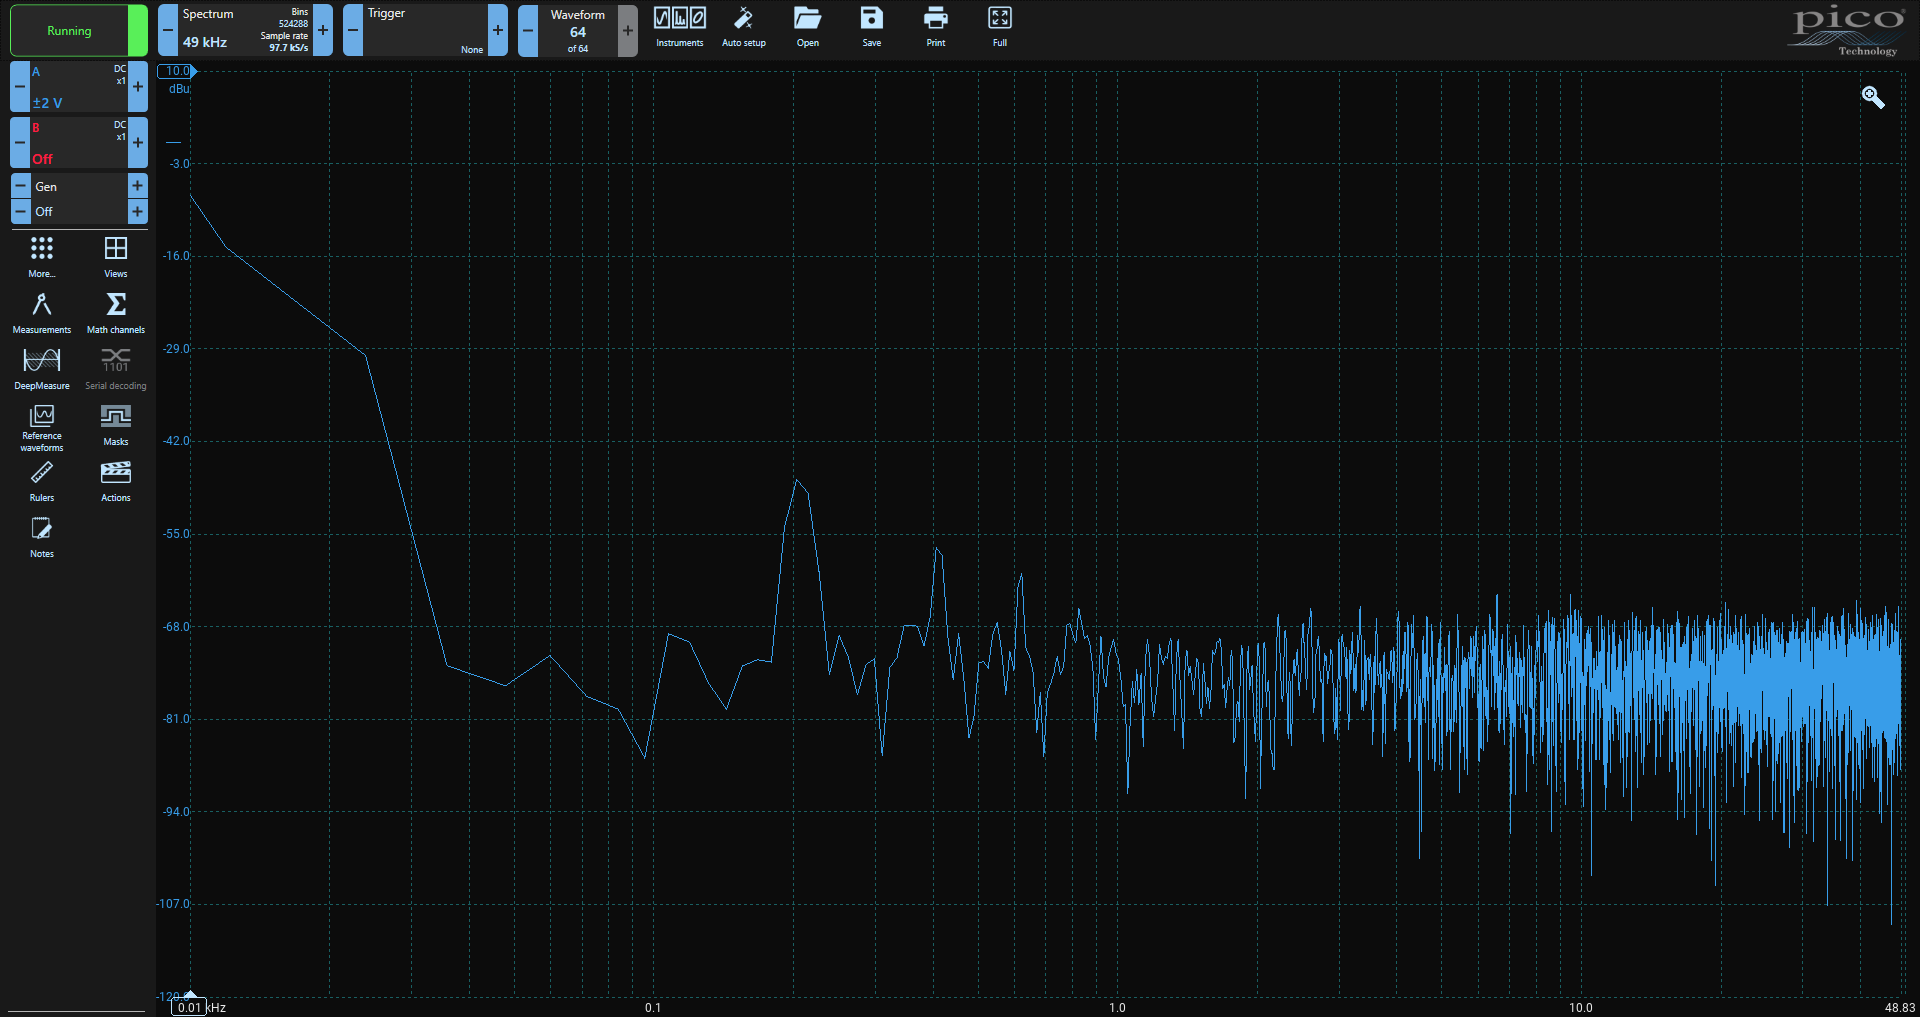
\includegraphics[width=0.99\textwidth]{figures/lospeed_biprop.png}
        \caption{Bi-Propeller}
        \label{fig:lospeed_biprop}
    \end{subfigure}
    % subfigure
    \begin{subfigure}{0.99\textwidth}
        \centering
        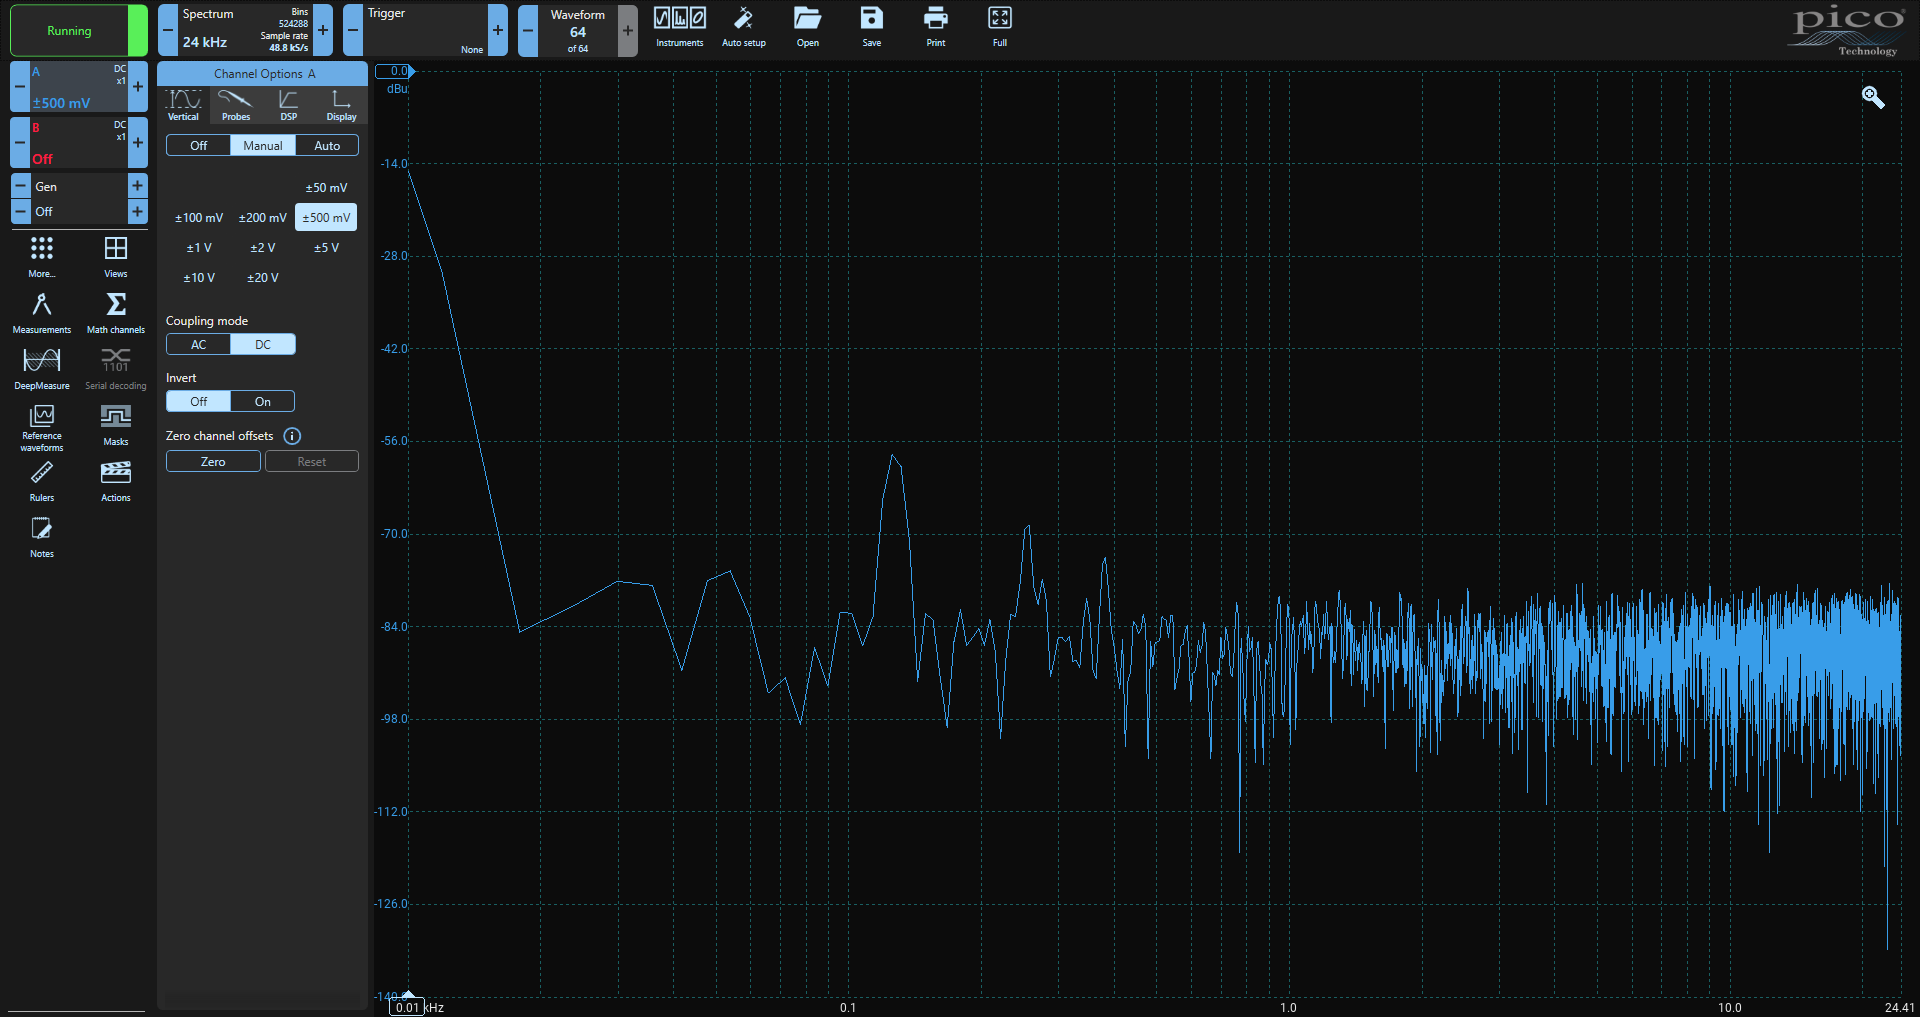
\includegraphics[width=0.99\textwidth]{figures/lospeed_toroid.png}
        \caption{Toroidal propeller}
        \label{fig:lospeed_toroid}
    \end{subfigure}
    \caption{Noise spectrum of propellers at low speed}
    \label{fig:noise_spectrum_lospeed}
\end{figure}

\section{Discussion}



\subsection{Acoustics}

The noise measured by the microphone, close to the propeller, was observed to be very directional.
The far field noise could not be measured due to lack of sensitivity and presence of background noise.
Noise measurements were also poor due to poor acoustics with some reflective surfaces, (e.g. table) close to the propellers.



\section{Conclusion}

\end{document}
